\documentclass[12pt]{article}
\usepackage{times, graphicx, epsfig, amsmath, color}
\usepackage{subfigure}
%sets 1in margins on letterpaper
\setlength\textwidth{6.5in}
\setlength\textheight{9.0in}
\setlength\topmargin{-0.5in}
\setlength\oddsidemargin{0.0in}
%\setlength\evensidemargin{-0.25in}
\renewcommand{\baselinestretch}{1.0}
\newcommand{\denselist}{\itemsep -1pt}
%\newcommand{\denselist}{\itemsep -3pt}
%\renewcommand{\theenumi}{\roman{enumi}} 
%\title{Learning to Track - Ideas}

\title{16-720 Computer Vision, Fall 2008 -- Assignment 6}
\author{Due: Thursday $4^{th}$ December 2008 at midnight}
\date{}
\begin{document}
\maketitle
\section{Image Segmentation}
In computer vision, image segmentation is often used as a preprocessing step for higher level tasks such as
object detection and object recognition. Therefore, one objective of image segmentation is to divide an image
into a set of meaningful regions which are good enough for subsequent tasks. In this homework, you will have to implement a segmentation algorithm and use it to segment a set of provided images. Unlike the previous homeworks, you will not be restricted to implement an existing paper or algorithm. 


On the course webpage, you can download the dataset that we are going to use for this homework. This dataset consists of 40 images; each image contains a single horse which is considered as the foreground object. The first row of Figure~\ref{fig:figure} displays some of these images. Your tasks for this homework are:
\begin{itemize}\denselist
	\item Come up with certain features (\textsl{e.g.} color, edge, texture) that work well with the
provided data.
	\item Design and implement an image segmentation algorithm.
	\item Produce the segmentation results for the provided images.
\end{itemize}
\begin{figure}
	\centering
		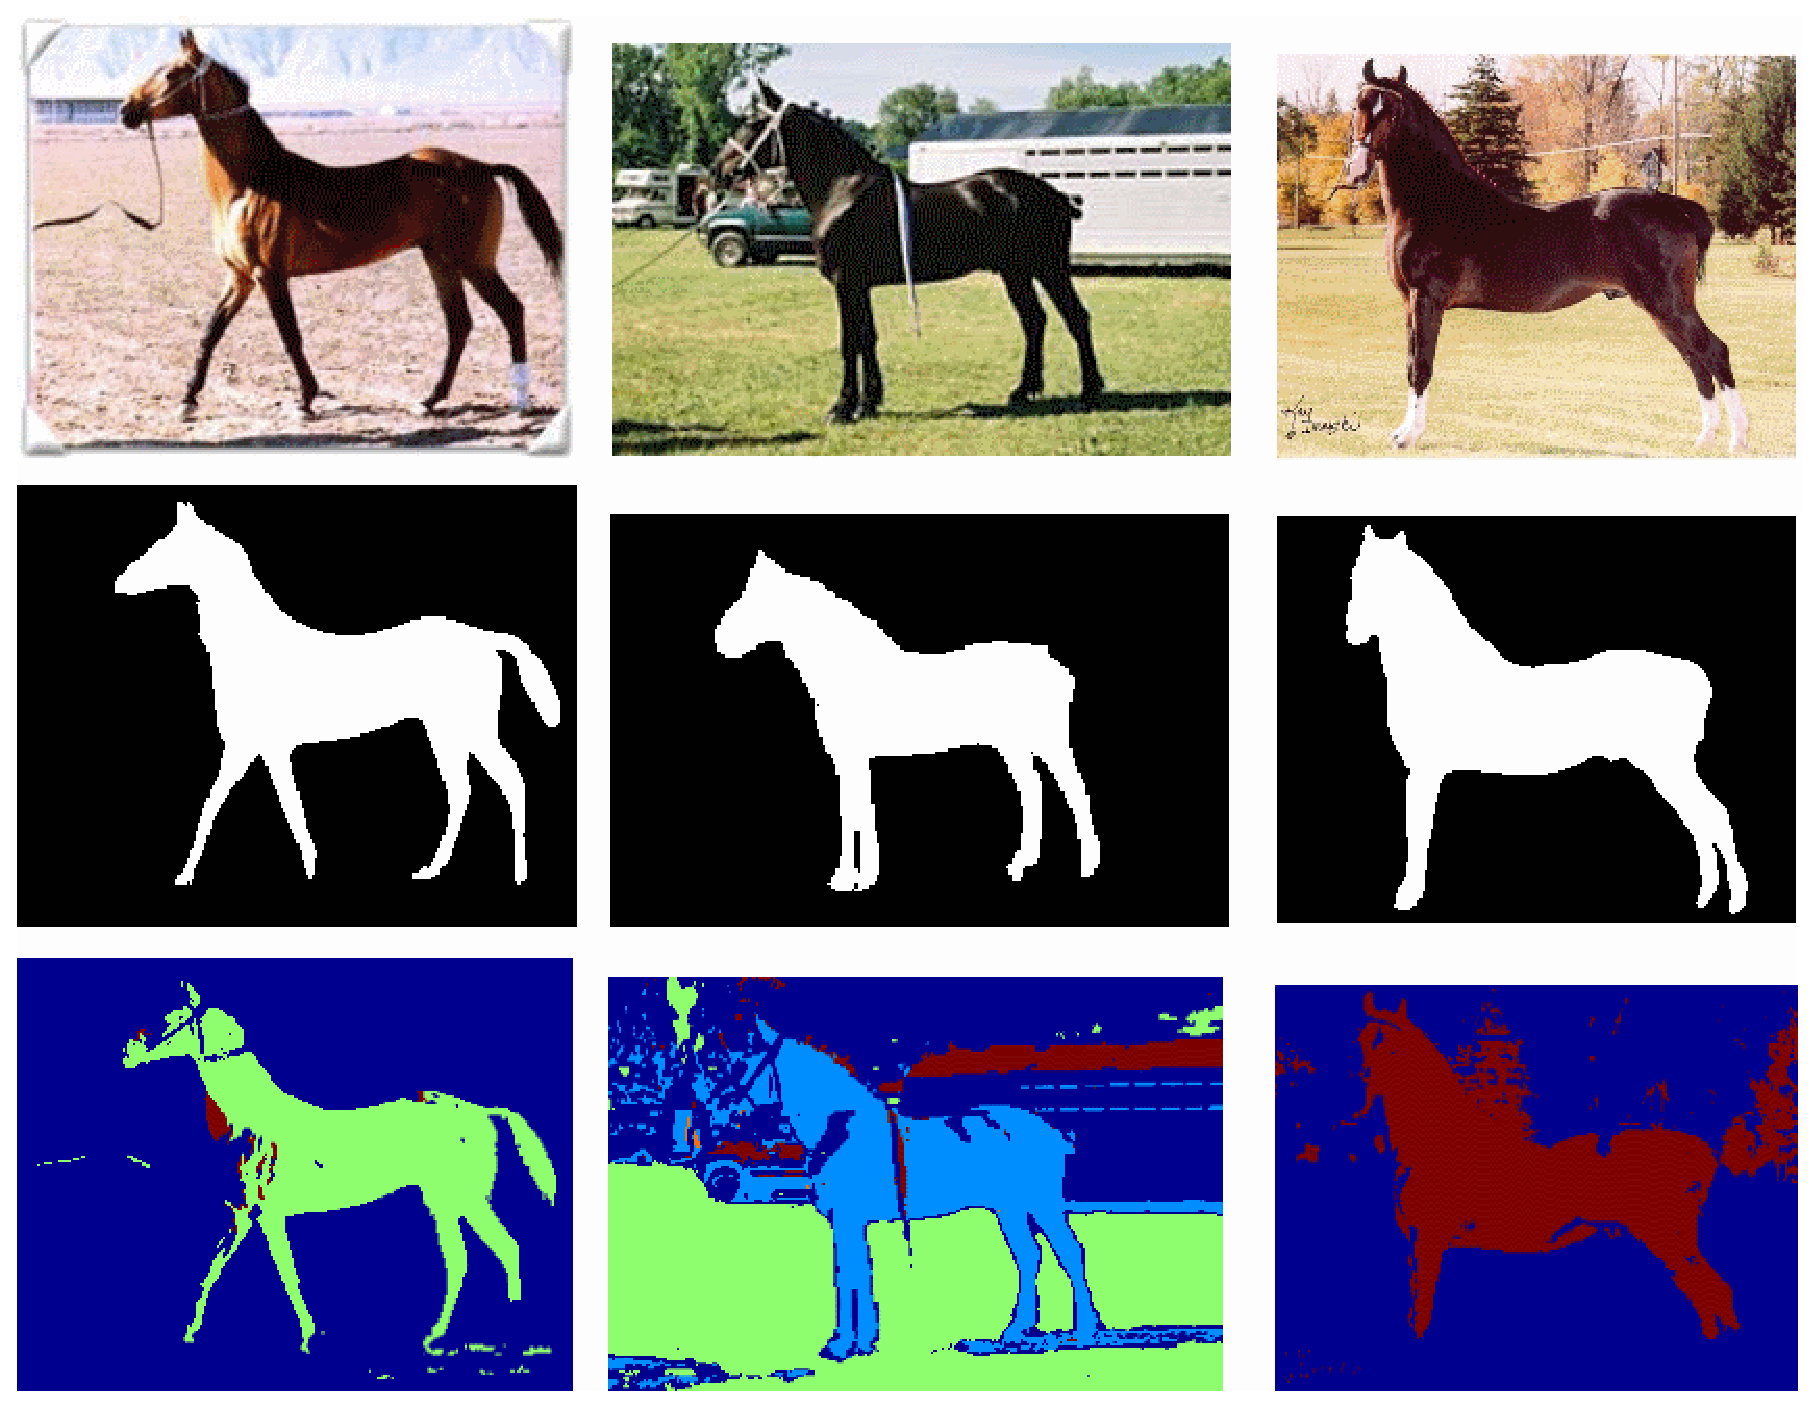
\includegraphics[width=1.00\textwidth]{./figures/figure.EPS}
	\caption{Several examples for input and output images. First row: several input images. Second row: the groundtruth foreground masks for the corresponding images in the first row. Third row: segmentation results of our SIMPLE segmentation algorithm without too much tuning; pixels of the same segment have the same color; different segments are assigned different colors. Our algorithm is based on \textsl{Mean Shift} in the Luv color space.}
	\label{fig:figure}
\end{figure}


%Your tasks are to design and implement an image segmentation algorithm that work best for certain classes of objects. In particular, for this homework, we are interested in horse segmentation. You will work with the data which comes with this homework. This dataset contains 50 images and their segmentation masks. Each image contains a single horse which is considered as the foreground object. The goal is to do your best on the foreground objects while achieving acceptable results in the background.
%
%
%Your task is to design and implement an
%
%
%come up with certain features (\textsl{e.g.} color, edge, texture) that work best with the
%provided data and design a segmentation algorithm. T
%
%We provide a set of horse images together with the segmentation masks. 
%a set of provided images. The images can be downloaded from the course webpage. Each image contains a single horse which is considered as the foreground object for that image. Your task is to come up with certain features (\textsl{e.g.} color, edge, texture) that best fit with the
%data and then design a segmentation algorithm. The goal is to do your best on the foreground
%objects, while achieve acceptable results in the background.


You should be able to finish this homework based on the materials covered in class. You are encouraged to propose your own algorithm. You can also search reference papers for state of the art techniques. If you choose to implement an  algorithm from existing papers, please cite them in your write-up.


\subsection{Algorithm design (40 points)}

%To finish this homework, you can use any material covered in this course. Although you are allowed to
%search reference papers for the state of art techniques, you should be able to finish this homework based
%on the materials covered in class. And you are encouraged to propose your own algorithms. If you do
%choose to implement an existing algorithm from a paper, please cite it in your write-up.
\vskip 0.25cm
\noindent\textbf{Q1}: Briefly describe your segmentation algorithm. You need to highlight the intuitions/ideas/theories underlying it. To help people (including yourself) understand your algorithm, it is helpful to
draw a graph showing the processing pipeline of your system.

\vskip 0.25cm
\noindent\textbf{Q2}: List the features used by your algorithm, explain why you think they are suitable for this task.



\subsection{Implementation (30 points)}
%\subsection{Datasets}
%In the dataset we provide you, there are labels for all the images. These labels are not perfect, for example
%the boundaries of the labels might not exactly correspond with boundary of objects. They might help
%your algorithm in some way, but you are not required to use these labels.
%For each image there is a corresponding .mat �le that contains a pixel-wise labeling of the image. (Ex-
%ample: image 2 10 s.bmp and annotation 2 10 s GT.mat) Loading the annotation �le will load a variable
%groundtruth into the workspace. groundtruth is an image whose dimensions match the dimensions of the
%original image. The pixels will contain one of the following values 0,1,2,3,4,5. An example annotation is
%shown in Figure 1 \& 2. Tree regions are represented as 1, Grass is represented as 2, Building is represented
%as 3, Cow is represented as 4, and Car is represented as 5. All remaining pixels are labeled as 0.
%
%Q3: If you are using the labels, in what way are you using them? If you are not using them, you do not
%need to answer this question.


%You can use all the images in whatever way you want to tune your algorithm. However, you need to provide a brief
%description of how you are making use of the images in your final write up.

\noindent\textbf{Q3}. Write the following function:

\verb|imSegment(input_image_list, path_to_output_directory)|

Running this function will automatically perform image segmentation on a set of images and output the results to a specified directory. \verb|input_image_list| is a cell array of strings that specify the full path of images that one wants to perform segmentation. We have given you an example stored in \textsl{imglist.mat}. Loading this file, you will have a variable called \textsl{imglist} in the Matlab workspace. The other input argument, \verb|path_to_output_directory|, is the output directory to store segmentation results. For each input image, your function needs to generate an output segmentation image. The output image must clearly show the segmentation results. Each segment must be associated with one unique color; different segments must be given different colors. The last row of Figure~\ref{fig:figure} shows some examples of output segmentation images. These images are generated by our simple image segmentation algorithm which is based on Mean Shift on the Luv color space. 
The name of the output file should only differ from the input file by the suffix \textsl{\_seg}. For example, if the input image is \textsl{image-032.png}, the output must be named \textsl{image-032\_seg.png} and placed in the directory  \verb|path_to_output_directory|.


%As a way to visually inspect the results, please save a label file for each
%input image. This output file should be the same format as the groundtruth file we described in Section
%1.2.1. Loading this file will load a variable called seg\_result into the workspace, which contains the
%labels defined the same as in the groundtruth file. Name the output file as: \textsl{*\_seg.mat}, where * stands for
%the original input image filename. For example, if the input image is: \textsl{image099.jpg}, the corresponding
%output file will be: \textsl{image099\_seg.mat}.

If your code requires pre-computed data (e.g. parameters, classifiers) that cannot be conveniently stored in the  code, you can store them in \textsl{.mat} files in the same directory with your code. When called, your function must automatically load any necessary data. 

\subsection{Experiments and tuning (30 points)}

\noindent\textbf{Q4}. Run your algorithm on the images listed in \textsl{imglist.mat}, and submit the segmentation results together with your code. 

\vskip 0.25cm
\noindent\textbf{Q5}. As with most computer vision applications, your implementation might not work right away. You are expected to spend a substantially amount of time tuning your function (e.g. size of filters, threshold). To answer this question, you will have to describe how you tune your algorithm.

You are free to used all the images for tuning. You can also use the foreground masks that come with the homework (the second row of Figure~\ref{fig:figure} shows some examples of foreground masks). One way to use these foreground masks is to design a quantitative evaluation and use it for automatic tuning. 
However, you are not required to do so. Yon can tune your method by qualitative evaluation. Whatever method you choose, you have to document it when answering this question.


%
%
%Design a procedure to evaluate the results you get. You might want to design it in a way that can emphasize the differences between your algorithm and others, and show why your algorithm is better.



%\noindent\textbf{Q4}: In which way are you using the images that we have provided you to tune your algorithm?
%
%\noindent\textbf{Q5}: Describe briefly the functionality of your evaluation methods.


%\subsection{Discussion (30 points)}
%Based on the evaluation section, briefly discuss how your algorithm is performing by answering the following questions.
%
%Q6: When you were designing the algorithm, what did you expect for the performance, and what part of
%your hypothesis were proved correct by the results?
%
%Q7: More importantly, if there is any, which part of your hypothesis were proved wrong, and how you
%interpret that? Can you give several examples?

\subsection{Hints}
\begin{itemize}\denselist
	\item Your algorithm does not need to be complicated.
	\item Perfect foreground segmentation is NOT required. We are only looking for implementations that provide sensible segmentation results. However, part of your grade for this homework will reflect the relative performance of your algorithm. 
	\item Computational time is not the primary consideration in this homework. However, it should be fast enough
for you to carry out repeatable experiments so that you have time to tune the program. Try to start or tune your algorithm with smaller subset of images first. 
\item Avoid loops in Matlab, practice more with vectorization techniques. 
\end{itemize}

\section{What to submit?}

\begin{itemize}\denselist
\item A file \textbf{\textsl{writeup.xxx}}, where \textbf{\textsl{xxx}} is the extension of the writeup file. The only acceptable file formats are \textsl{pdf, doc}, and \textsl{txt}. This file should contains the answers to all the questions and anything you want us to know about your algorithm. 
\item All source files and any \textbf{\textsl{.mat}} files you your functions require. Comments are greatly appreciated. 
\item The results of your image segmentation algorithm on the set of provided images. The results should be placed in a directory called \textbf{\textsl{results}}. Furthermore, make sure that this directory ONLY contain the results that we asked; no extra junk please. If you think your algorithm is impressive and you would like to show us other results (e.g. for different types of images, using alternative parameters), please put them in a separate directory called \textbf{\textsl{results2}}. If you do include extra results, please document them in the write-up.
\item DO NOT put any non-result (segmentation images) that we do not ask for in the \textbf{\textsl{results}} directory.
\item DO NOT submit the images that we provide.
\item DO NOT include your code in the write-up.
\end{itemize}


%\input{definitions.tex}

%\bibliographystyle{../../../../MyNotes/splncs-new}
%\bibliography{../../../../MyNotes/pubs}
\end{document}
 